\section{Введение}

\subsection{Комбинаторные виды}
Комбинаторные виды (\emph{species}) были введены Жуаялем в 1980 году \cite{J1}.
Они дают универсальный аппарат изучения помеченных (labeled) и
непомеченных (unlabeled) структур, и являются развитием идеи производящих
функций. О комбинаторных видах можно говорить на нескольких языках: категорном,
комбинаторном и на языке теории представлений. Последний наиболее часто
встречается в литературе, хотя автору он кажется наимение выразительным.
Во введении изложено начало теории комбинаторных видов. Основным источником
информации про комбнаторные виды является \cite{BergTrees}.
\subsubsection{Определение}
Рассмотрим категорию $\B$ --- группоид конечных множеств. Она эквивалентна
группоиду, объекты которого пронумерованы неотрицательными целыми числами и
$Hom(n, n) = S_n$.
\begin{definition}
Комбинаторным видом (species) называется функтор $$F:\B \rightarrow \Set$$
\end{definition}

Задать такой функтор, это то же самое что для каждого $n \in
\mathbb N$ задать множество $F[n]$ с действием группы $S_n$. В комбинаторике
такая ситуация возникает, когда мы рассматриваем явно определнные каким-либо
образом структуры на конечных множествах. Например: линейные порядки,
циклические порядки, деревья. Действие $S_n$ ествественно возникает из
перестановок исходных точек.
\begin{example}
Вид $\E$ --- вид множесто (без дополнительной структуры). Он
сопоставляет набору точек одно множество, состоящие из этих точек, 
$\E[n] =\{*\}$. Все элементы $S_n$ переходят в тождественное отображение. 
\end{example}
\begin{example}
$\mathbf C$ --- циклический порядок. Сопоставляет набору из $n$ точек
$(n-1)!$ возможных циклических порядков на них. 
\end{example}
\begin{example}
Линейный порядок $\mathbf L$ сопоставляет $n!$ линейных
порядков. 
\end{example}
\begin{example}
$\E_e$ --- сужение $\E$ на четные множества. То есть для четных
$n$, совпадает с $\E$, а для нечетных $\emptyset$. 
Аналогично $\E_o$ --- сужение на нечетные.
\end{example}
\begin{example}
На картинке \ref{pic:3-rooted-trees} изображен вид <<корневые
деревья с 3 вершинами>> (без какого-либо порядка на потомках).
\end{example}

\begin{figure}
\begin{center}
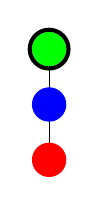
\begin{tikzpicture}
\draw (0pt, 0pt) -- (0pt, -20pt);
\draw (0pt, -20pt) -- (0pt, -40pt);
\draw[color=green, fill] (0pt,0pt) circle (6pt);
\draw[color=black, line width=1.5pt] (0pt,0pt) circle (7pt);
\draw[color=blue, fill] (0pt, -20pt) circle (6pt);
\draw[color=red, fill] (0pt, -40pt) circle (6pt);
\end{tikzpicture}
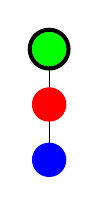
\begin{tikzpicture}
\draw (0pt, 0pt) -- (0pt, -20pt);
\draw (0pt, -20pt) -- (0pt, -40pt);
\draw[color=green, fill] (0pt,0pt) circle (6pt);
\draw[color=black, line width=1.5pt] (0pt,0pt) circle (7pt);
\draw[color=red, fill] (0pt, -20pt) circle (6pt);
\draw[color=blue, fill] (0pt, -40pt) circle (6pt);
\end{tikzpicture}
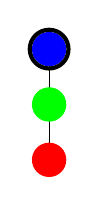
\begin{tikzpicture}
\draw (0pt, 0pt) -- (0pt, -20pt);
\draw (0pt, -20pt) -- (0pt, -40pt);
\draw[color=blue, fill] (0pt,0pt) circle (6pt);
\draw[color=black, line width=1.5pt] (0pt,0pt) circle (7pt);
\draw[color=green, fill] (0pt, -20pt) circle (6pt);
\draw[color=red, fill] (0pt, -40pt) circle (6pt);
\end{tikzpicture}
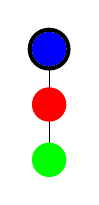
\begin{tikzpicture}
\draw (0pt, 0pt) -- (0pt, -20pt);
\draw (0pt, -20pt) -- (0pt, -40pt);
\draw[color=blue, fill] (0pt,0pt) circle (6pt);
\draw[color=black, line width=1.5pt] (0pt,0pt) circle (7pt);
\draw[color=red, fill] (0pt, -20pt) circle (6pt);
\draw[color=green, fill] (0pt, -40pt) circle (6pt);
\end{tikzpicture}
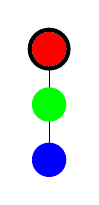
\begin{tikzpicture}
\draw (0pt, 0pt) -- (0pt, -20pt);
\draw (0pt, -20pt) -- (0pt, -40pt);
\draw[color=red, fill] (0pt,0pt) circle (6pt);
\draw[color=black, line width=1.5pt] (0pt,0pt) circle (7pt);
\draw[color=green, fill] (0pt, -20pt) circle (6pt);
\draw[color=blue, fill] (0pt, -40pt) circle (6pt);
\end{tikzpicture}
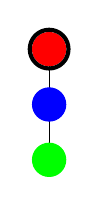
\begin{tikzpicture}
\draw (0pt, 0pt) -- (0pt, -20pt);
\draw (0pt, -20pt) -- (0pt, -40pt);
\draw[color=red, fill] (0pt,0pt) circle (6pt);
\draw[color=black, line width=1.5pt] (0pt,0pt) circle (7pt);
\draw[color=blue, fill] (0pt, -20pt) circle (6pt);
\draw[color=green, fill] (0pt, -40pt) circle (6pt);
\end{tikzpicture}
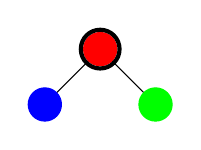
\begin{tikzpicture}
\draw (0pt, 0pt) -- (-20pt, -20pt);
\draw (0pt, 0pt) -- (20pt, -20pt);
\draw[color=red, fill] (0pt,0pt) circle (6pt);
\draw[color=black, line width=1.5pt] (0pt,0pt) circle (7pt);
\draw[color=blue, fill] (-20pt, -20pt) circle (6pt);
\draw[color=green, fill] (20pt, -20pt) circle (6pt);
\end{tikzpicture}
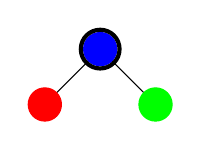
\begin{tikzpicture}
\draw (0pt, 0pt) -- (-20pt, -20pt);
\draw (0pt, 0pt) -- (20pt, -20pt);
\draw[color=blue, fill] (0pt,0pt) circle (6pt);
\draw[color=black, line width=1.5pt] (0pt,0pt) circle (7pt);
\draw[color=red, fill] (-20pt, -20pt) circle (6pt);
\draw[color=green, fill] (20pt, -20pt) circle (6pt);
\end{tikzpicture}
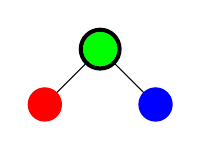
\begin{tikzpicture}
\draw (0pt, 0pt) -- (-20pt, -20pt);
\draw (0pt, 0pt) -- (20pt, -20pt);
\draw[color=green, fill] (0pt,0pt) circle (6pt);
\draw[color=black, line width=1.5pt] (0pt,0pt) circle (7pt);
\draw[color=red, fill] (-20pt, -20pt) circle (6pt);
\draw[color=blue, fill] (20pt, -20pt) circle (6pt);
\end{tikzpicture}
\end{center}
\caption{корневые деревья с 3 вершинами}
\label{pic:3-rooted-trees}
\end{figure}

Можно рассмотреть функтор $I:\Set \rightarrow Vect$, который сопоставляет
множеству векторное пространство, базис которого это множество.
Тогда $F \circ I: \B \rightarrow Vect$ --- сопоставляет каждому $n$
перестановочное представление группы $S_n$. При таком подходе, значение
характера этого представления $\chi(\sigma)$, это количество структур,
неподвижных относительно $\sigma \in S_n$.

\subsubsection{Сложение комбинаторных видов}
Сумму двух species $F$ и $G$ определим как поточечную сумму функторов.
На комбинаторном языке это будет означать <<либо структура типа $F$, либо
структура типа $G$>>. $(F + G)[n] = F[n] \coprod G[n]$ с покомпонентным
действием $S_n$.
\begin{example}
$\mathbb E = \mathbb E_e + \mathbb E_o$
\end{example}
\begin{example}
Любой вид $F$ можно разложить в такую сумму $F =
F_{1} + F_{2} + F_{3} + \dots$, где $F_{i}$ --- сужение $F$ на $i \in \mathcal
B$. Значение $F_{i}$ на $j \neq i$ равно $\emptyset$.
\end{example}

\subsubsection{Произведение комбинаторных видов} 
Определим произведение по Коши комбинаторных видов. По определению задать на
конечном множестве структуру типа $F \cdot G$ означает разбить множество точек 
на две части (всевозможные) и на первом ввести структуру типа $F$,
на втором --- типа $G$. 
$$(F \cdot G)[X] = \coprod\limits_{X_1 \coprod X_2 =
X}F[X_1] \times G[X_2]$$


C категорной точки зрения произведение по Коши возникает из тензорного
произведения на категории $\B$, которое на объектах задается как $n \otimes m =
(n + m)$, на морфизмах при помощи вложения $S_n \times S_m \hookrightarrow
S_{n+m}$ (все такие вложения сопряжены).
Известна конструкция свертки функторов из $\mathcal C$ в $\Set$, где
$\mathcal C$ --- моноидальная категория с копроизведениями
\href{http://nlab.mathforge.org/nlab/show/Day+convolution}{[Day
convolution \cite{Day}]}.


На языке теории представлений $F[n+m]$ как множество с действием группы
$S_{n+m}$ равно индуцированному представлению $Ind \uparrow_{S_n \times S_m}
^{S_{n+m}} F[n]\times F[m]$.

\begin{example}
$\E \times \E_1$ --- множество с выделенной точкой.
\end{example}
\begin{example}
$\mathbf C^2$ --- (упорядоченная) пара циклов.
\end{example}

\subsection{Композиция комбинаторных видов}
Кроме сложения и умножения на species можно ввести операцию композиции.
По определению задать на конечном множестве структуру типа $F \circ G$ означает
разбить множество точек на части (всевозможные), на частях (как новых точках)
ввести структуру типа $F$, а на каждой части --- типа $G$. Иначе говоря, <<раздуть>>
каждую точку структуры типа $F$ в структуру типа $G$.
$$
(F \circ G)[X] =
\coprod\limits_{\coprod\limits_i X_i = X} F[\{X_i\}_i] \times
(\coprod\limits_{i} G[X_i]) 
$$

\begin{remark}
\label{rem:finit}
Определение species не предполагает конечности $F[n]$, однако цикленный индекс
(см. раздел \ref{sec:cycle}) можно писать только для таких видов. Класс таких
species не замкнут относительно композиции. Поскольку при подстановке
species $F$, для котогоро $F[0] \neq \emptyset$ можно выделить сколько угодно пустых
частей. Поэтому в дальнейшем в записи $F \circ G$, мы будем неявно предполагать
что внутренний операнд <<сужен>> на $\mathbb N_{+}$.
\end{remark}

\begin{example}
$\E_1 \circ F = F$, $F \circ \E_1 = F$. $\E_1$ является нейтральным элементом в
моноиде species по композиции.
\end{example}
\begin{example}
$\E_2 \circ \mathbf C$ --- (неупорядоченная) пара циклов.
\end{example}
\begin{example}
$\E \circ \E$ --- структура разбиения множества.
\end{example}
\begin{example}
$\E \circ \mathbf C = \mathbf S$ --- структура перестановки.
Буквально перестановка --- это набор циклов.
\end{example}

Для того, чтобы ввести композицию на категорном языке нам
понадобится дополнительная конструкция: аналитический функтор.
\subsubsection{Аналитический функтор комбинаторных видов}
Аналитический функтор (введен Жуаялем в \cite{J2}) $\mathcal F$ соответствует
species $F$. Вводить его можно разными способами, мы ограничимся универсальным
свойством и явной конструкцией. 
\begin{definition}
Аналитический функтор является левым расширением по Кану функтора $F$
относительно $i$.

\begin{tikzpicture}
\label{comm:an}
	\node (B) {$\B$};
	\node (S1) [below of=B] {$\Set$};
	\node (S2) [right of=B, node distance=3cm] {$\Set$};
	\draw [right hook->] (B) to node [swap] {$i$} (S1);
	\draw [->] (B) to node {$F$} (S2);
	\draw [->] (S1) to node [swap] {$\mathcal F$} (S2);	
\end{tikzpicture}
\end{definition}

Эта диаграмма не является коммутативной, а коммутативна лишь настолько,
насколько может быть коммутативной диаграмма подобного вида. А именно,
существует естественное преобразование  $\kappa \colon F \rightarrow i \circ
\mathcal F$, обладающее следующим универсальным свойством:
для любого функтора $M \colon \Set \rightarrow \Set$ и морфизма функторов $\eta
\colon F \rightarrow i \circ M$ этот морфизм пропускаеться через $\mathcal F$ при помощи $\kappa$.

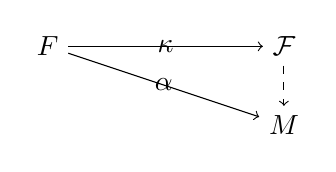
\begin{tikzpicture}
\label{comm:an-uni}
	\node (F) {$F$};
	\node (Fm) [right of=F, node distance=3cm] {$\mathcal F$};
	\node (M) [below of=Fm] {$M$};
	\draw [->] (F) to node {$\kappa$} (Fm);
	\draw [->] (F) to node [swap] {$\alpha$} (M);
	\draw [->, dashed] (Fm) to node [swap] {} (M);
\end{tikzpicture}


Явная конструкция для аналитического функтора.
\begin{equation}
\label{eq:an}
	\mathcal F(A) = \sum\limits_n F[n] \times A^n / S_n
\end{equation}
Получается из общекатегорных соображений о продолжении функтора на категорию
предпучков по непрерывности (непрерывность понимается в смысле свойства
сохранения копределов). Теория кратко изложена на 2-4 страницах \cite{DoldKan}. Это
расписанная формула под диаграммой на странице 4 (копредел по категории $D_G$).
Так же доказательство написано в \cite{BergTrees}.

\begin{remark}
\label{rem:color}
У аналитического функтора для типа структуры $F$ имеется прозрачная
комбинаторная интерпретация.
Если трактовать множество $A$ как набор цветов,
то значение аналитического функтора $\mathcal F(A)$ трактуется как множество структур типа $F$
раскрашенных в цвета из $A$.
\end{remark}

\subsubsection{Композиция аналитических функторов комбинаторных видов}
\begin{theorem}
Композиция аналитических функторов $\mathcal F \circ \mathcal G$ является
аналитическим функтором для $F \circ G$.
\end{theorem}
\begin{proof}
Набросок. Согласно конструкции $\mathcal F(\mathcal
G (A)) = \sum\limits_k F[k] \times (\sum\limits_m G[m] \times A^m / S_m)^k /
S_k = \sum\limits_n \sum\limits_{k, m_1 + \dots + m_k = n} F[k] \times
(\coprod\limits_{i} G[m_i]) \times A^n / S_n$.

Строгое доказательство см. в \url{http://arxiv.org/pdf/math/9811127v1.pdf}
(Lemma 2.5) [это еще и про цикленные индексы]
\end{proof}

\subsubsection{Другой взгляд на композицию аналитических функторов}
Дело в том, что композиция комбинаторных видов --- это в некотором смысле
частный случай аналитического функтора, только не со значениями в $Set$,
а со значениями в $\Species = \Hat \B$.

А именно, для любой моноидальной категории $\mathcal C$ со всевозможными
копределами и объекта $A$ из $\mathcal C$, функтор из $\mathcal B$ в $\mathcal
C$, который $1$ отправляет в $A$, а $n$ отправляет в $A^{\otimes n}$ (тензорная
степень), можно <<продолжить по непрерывнoсти>> (видимо расширение Кана) до
функтора из категории предпучков на $\mathcal B$ со значениями в $\mathcal C$
\cite{Durov}. В этой работе Дурова этот фнктор обозначается $\Phi_A$.

В случае когда $\mathcal C = Set$, получаем
$\Phi_A(F)=\mathcal F(A)$. В случае, когда $\mathcal C = \Species$, получаем
$\Phi_G(F)=F \circ G$. То есть можно определить композицию, как функтор
$G \mapsto F\circ G$ при помощи $\Phi_G$. Надо только проверить функториальность
по $G$ (в обозначении $\Phi_G$, буква $G$ обозначает постоянный параметр, а в
аналитеческом функторе --- это переменный аргумент).
При таком взгляде на подстановку теорема о композиции становится почти тавтологией.

\subsubsection{Цикленный индекс}
\label{sec:cycle}
%Процедура декатегорификации не имеет строго математического смысла, так же как
%и процедура квантования.
%Сейчас мы предложим процедуру, которая, стартуя с обычных species,
%на выходе дает классический цикленный индекс/фробениусову характеристику.
%Затем мы попытаемся аналогические действия провести и в гипероктаэдральном
% случае.
%Декатегорификацией моноидальной категории $\mathbb B$ является моноид классов
% изоморфизма объектов категории $\mathbb \B$, то есть моноид натуральных чисел по сложению.
%Декатегорификкацией $\widehat{\mathbb \B}$ естественным образом оказывается
%моноидная алгебра с коэффициентами из $\mathbb Z$ для моноида $\mathbb N$, то
% есть кольцо многочленов $Z[X]$.
%(Правда это не то, что мы хотели. Чтобы получить цикленный индекс надо
% декатегорифицировать саму операцию подстановки и аналитический функтор).
% [TODO: этот таинственный абзац стоит переписать]

Будем рассматривать только species, конечные в смысле замечания
\ref{rem:finit}.
Хочется используя идею подсчета с весом, написать аналог производящей функции
для покрашенных (в смысле замечания \ref{rem:color}) структур. Цветам
сопоставим переменные $x_1, x_2, x_3, \dots$. Раскрашенной структуре с
раскраской $\{x_{i_1}, x_{i_2}, \dots, x_{i_k}\}$ сопоставим моном $x_{i_1} x_{i_2} \dots x_{i_k}$.  
Например, расскраске в которой 2 первых цвета и 1 второй соответсвует моном
$x_1^2x_2$. 
Суммируя по всем расскрашенным структурам из формулы \ref{eq:an}, мы получим
симметрическую (от $x_1, x_2, x_3, \dots$) функцию. Коэффициент
при каждом мономе --- это число раскрашенных структур с заданной расскраской. 

Введем некоторые обозначения 
$\lambda = (\lambda_1, \lambda_2, \lambda_3, \dots) \vdash n$ --- разбиение.
$\sigma$ --- перестановка цикленного типа $\lambda$. $z_\lambda$ --- индекс
класса сопряженности $\sigma$.
$\chi$ --- характер (перестановочного) представления заданного $F$.
$\psi^{\lambda} = 
(x_1^{\lambda_1} + x_2^{\lambda_1} + x_3^{\lambda_1} + \dots)
(x_1^{\lambda_2} + x_2^{\lambda_2} + x_3^{\lambda_2} + \dots)
(x_1^{\lambda_3} + x_2^{\lambda_3} + x_3^{\lambda_3} + \dots)
\dots$.

\begin{statement}
Фробениусовой характеристикой или цикленным индексом species $F$ будем называть
симметрическую функцию:
\begin{equation}
\label{eq:fr}
\mathcal Z_F =
\sum_{n}\frac{1}{n!}\sum_{\sigma \in S_n}\chi(\sigma)\psi^{\lambda(\sigma)} =
\sum_{n, \lambda \vdash n}\chi(\sigma_{\lambda})
\frac{\psi^{\lambda}}{z_{\lambda}}
\end{equation}
Коэффициент при мономе $x_{i_1} x_{i_2} \dots x_{i_k}$ равен числу
раскрашенных структур с расскраской $\{x_{i_1}, x_{i_2},
\dots, x_{i_k}\}$.

\end{statement}
\begin{proof}
По Лемме Бернсайда количество орбит равно усредненному по всем элементам
группы числу неподвижных точек. Чтобы раскрашенная структура была неподвижна под
действием перестановки $\sigma$ нужно, чтобы во-первых она была неподвижна как
нераскрашенная структура, а во-вторых расскраска должна переходить в себя.
Тогда первое условие дает нам сомножитель
$\chi(\sigma)$. Второе условие требует покраски каждого
цикла в один и тот же цвет.
\end{proof}

\begin{example}
$\mathcal Z_{\E_1} = \psi^1$
\end{example}

\begin{example}
$\mathcal Z_{\E_2} = \frac{1}{2}((\psi^1)^2 + \psi^2)$
\end{example}

\begin{example}
$\mathcal Z_{\E} = e^{(\psi^1 + \frac{\psi^2}{2} + \frac{\psi^3}{3} +
\dots)}$. Доказательство смотри в \cite{BergTrees}.
\end{example}

\subsubsection{Плетизм цикленных индексов}
\begin{theorem}
Композиции аналитических функторов соответствует плетизм цикленных
индексов.
\end{theorem}
Чудесный факт заключается в том, что в декатегорификации
композиция соответствует простой формуле подстановки. Сейчас мы ее напишем и
приведем набросок доказательства. В качестве множества цветов $A$ рассмотрим
счетный набор цветов $x_1, x_2, x_3, \dots$ Цикленный индекс запишем
относительно базиса кольца симметрических функций $\psi^1, \psi^2, \psi^3, \dots$
\begin{statement}
\label{th:compos}
\begin{multline}
\label{eq:zfg}
	\mathcal Z_{F \circ G} (\psi^1, \psi^2, \psi^3, \dots) = \\
	\mathcal Z_F(
		\mathcal Z_G(\psi^1, \psi^2, \psi^3, \dots),
		\mathcal Z_G(\psi^2, \psi^4, \psi^6, \dots),
		\mathcal Z_G(\psi^3, \psi^6, \psi^9, \dots),
		\dots
	)
\end{multline}
\end{statement}
\begin{proof}
В композиции двух аналитических функторов получается, что цвета в которые мы
красим структуру $F$ это структуры типа $G$. То есть $\mathcal Z_{F \circ G} =
\mathcal Z_F(\psi_g^1, \psi_g^2, \psi_g^3, \dots)$, где $\psi_g^i = (g_1^i +
g_2^i + g_3^i + \dots)$, где $g_i$ --- перечисление всех структур типа $G$.
Нужно раскрыть переменные $g_i $ --- написать их относительно начальных цветов.
Формулу $\psi_g^i = \mathcal Z_G(\psi^i, \psi^{2i}, \psi^{3i}, \dots)$ легко
понять в переменных $x_1, x_2, x_3, \dots$. Мы должны покрасить $i$ кусков в
одну и ту же $G$--структуру. Значит каждый цвет $x_j$ в $\mathcal Z_G$ при
подстановке в $\psi^i$ заменяется на $x_j^i$.
\end{proof}
\begin{remark}
Формулу \ref{eq:zfg} можно специализировать для подсчета labeled--структур. То
есть покрашенных структур у которых нет двух одинаковых цветов в расскраске.
Соответсвующие мономы (в базисе $x_1, x_2, x_3, \dots$) возникают только при
раскрытии мономов вида $c(\psi^1)^k$ и коэффициент в них равен $ck!$ --- такой
же как при мономе с точностью до факториала. Этот факториал приводит к
необходимости рассматривать экспоненциальные производящие функции вместо
обычных. Можно занулить все остальные мономы подстановкой $\psi^1 = t, \psi^2 =
0, \psi^3 = 0, \psi^4 = 0$. Формула \ref{eq:zfg} примет вид $
\mathcal Z_{F \circ G} (t, 0, 0, \dots) =
	\mathcal Z_F(
		\mathcal Z_G(t, 0, 0, \dots), 0, 0, \dots
	)
$.
А значит для экспоненциальных производящих функции labeled-структур справедливо
равенство
\begin{equation}
\label{eq:comp}
(f \circ g) (t) = f(g(t))
\end{equation}
\end{remark}

\begin{example}
(Экспоненциальная) производящая функция для $\E$ это $e^x = 1 + x +
\frac{1}{2!}x^2 + \frac{1}{3!}x^3 + \dots$. А производящая функция для
непустых циклов $\mathbf C$ это $-log(1-x) = x + \frac{1}{2}x^2 +
\frac{1}{3}x^3 + \dots$.
А для $\mathbf S$ производящая функция это $\frac{1}{1-x} = 1 + x + x^2 + x^3 +
\dots$.
И действительно $e^{-log(1-x)} = \frac{1}{1-x}$.
\end{example}
